\part{Liquids}
\section{Newtonian and Non-Newtonian Liquids}
The definition of a Newtonian liquid is that $\sigma \propto \dot\gamma$, so the viscosity 
\begin{equation}
	\eta = \sigma / \dot\gamma
	\label{eq:newtonian_viscosity}
\end{equation}
is constant. Otherwise the liquid is non-Newtonian, and the viscosity is a function of shear rate, stress, or time.
The tensor for of equation \ref{eq:newtonian_viscosity} is
\[
	\sigma_{ij} = 2\eta D_{ij},
\]
where $D_{ij} = \frac{1}{2}(\partial_i u_j + \partial_j u_i)$ is the rate of deformation tensor.

\subsection{Extensional viscosity}
Start with imposing:
\[ u_x = \dot\gamma x \]
If incompressible: $\nabla\cdot u = 0 \therefore Tr(D) = 0$, so 
\[
	u_y = -\frac{1}{2}\dot\gamma y, \qquad
	u_z = -\frac{1}{2}\dot\gamma z.
\]
Then our \emph{deformation rate tensor} is
\begin{equation}
	D_{ij} = \tfrac12\dot\gamma \begin{bmatrix}
		2 & 0 & 0 \\
		0 & -1 & 0 \\
		0 & 0 & -1
	\end{bmatrix}.
	\label{eq:deformation_rate_tensor_extensional}
\end{equation}
For \emph{stress}, we have
\(
	\sigma_{ij} = -pI + 2\eta D_{ij}.
\)
In rheology, generally you don't care about pressure, so this simplifies to
\begin{equation}
	\sigma_{ij} = \eta \dot\gamma \begin{bmatrix}
		2 & 0 & 0 \\
		0 & -1 & 0 \\
		0 & 0 & -1
	\end{bmatrix}.
	\label{eq:stress_tensor_extensional}
\end{equation}
The rate of mechanical work per unit volume is
\[
\mathcal{P} = \sigma : D = \sigma_{ij}D_{ij}.
\]
For an incompressible fluid, $\sigma_{ij} = -p\delta_{ij} + \tau_{ij}$ and
$\mathrm{tr}(D)=0$, so pressure does no work and only deviatoric stresses
contribute to deformation. Using equations \ref{eq:deformation_rate_tensor_extensional} and \ref{eq:stress_tensor_extensional} we have
\[
\mathcal{P} = (\sigma_{xx}-\sigma_{yy})\dot\gamma,
\]
so $\sigma_{xx}-\sigma_{yy}$ is the stress driving extension. The
extensional viscosity is therefore defined as
\[
\eta_E = \frac{\sigma_{xx}-\sigma_{yy}}{\dot\gamma}.
\]
Plugging in the values from equation \ref{eq:stress_tensor_extensional} gives
\[
\eta_E = 3\eta.
\]
The \emph{Trouton ratio} is the ratio of extensional viscosity to shear viscosity:
\[	\text{Tr} = \frac{\eta_E}{\eta} = 3.
\]

\subsection{Shear viscosity}
Start with imposing:
\[ u_x = \dot\gamma y, \qquad
	u_y = 0, \qquad
	u_z = 0.
\]
Then our \emph{deformation rate tensor} is
\[
	D_{ij} = \tfrac12\dot\gamma \begin{bmatrix}
		0 & 1 & 0 \\
		1 & 0 & 0 \\
		0 & 0 & 0
	\end{bmatrix}.
\]

\subsection{Biaxial extension}
Start with imposing:
\[
	u_x = \dot\gamma x, \qquad
	u_y = \dot\gamma y, \qquad
	u_z = -2\dot\gamma z.
\]
Then our \emph{deformation rate} and \emph{stress} tensors are\footnote{
	Using $\sigma_{ij} = 2\eta D_{ij}$ and ignoring pressure.
}
\[
	D_{ij} = \tfrac12\dot\gamma \begin{bmatrix}
		2 & 0 & 0 \\
		0 & 2 & 0 \\
		0 & 0 & -4
	\end{bmatrix}
	\quad \text{and} \quad
	\sigma_{ij} = \eta \dot\gamma \begin{bmatrix}
		2 & 0 & 0 \\
		0 & 2 & 0 \\
		0 & 0 & -4
	\end{bmatrix}.
\]
\[
	\boxed{\eta_B = \frac{\sigma_{xx}-\sigma_{zz}}{\dot\gamma} = 6\eta}.
\]
\subsection{Intensity of dissapation}
\[
	A = \sigma : D = \sigma_{ij}D_{ij}.
\]
This can also be written in terms of the \emph{second invariant of the deformation rate tensor} $D_2$:
\[
	A = -4\eta D_2 \quad \text{where}\quad
	D_2 = \sum_{i,j} \dot\gamma_{ij}^2.
\]
Not sure if that is correct, I think the correct result is something more like
\[
	A = \sigma : D = 2\eta D : D = 2\eta \sum_{i,j} D_{ij}^2
	  = 4\eta D_2.
\]
where $D_2= \tfrac12 D:D$ is the \emph{second invariant of the deformation rate tensor}.

\section{Questions}

\subsection{3-1 Malkin}
Can viscosity be negative? Explain the answer.

\subsection{3-2 Malkin}
In measuring the viscous properties of the polymer solution, it appeared that the experimental data within the experimental range of shear rates can be fitted with the power-law equation (Eq. 3.3.4). Analyze the possibility of extrapolating this equation to the range of very high shear rates.

\textbf{Additional question.} Which kind of rheological behavior at high shear rates is expected in this case?

\subsection{3-3 Malkin}
What is the difference in stress relaxation of viscous liquids and viscoplastic materials?

\subsection{3-4 Malkin}
Can we expect that the values of the yield stress, $\sigma_Y$, found by treating a set of experimental data by means of Eqs. 3.3.7 to 3.3.9, are the same?

\subsection{3-5 Malkin}
Calculate shear stresses in the flow of liquid through a straight tube if the flow is created by the pressure gradient $\Delta p/L$ ($L$ is the length of a tube).

\textbf{Additional question.} Are the results valid for Newtonian liquid only?

\subsection{3-6 Malkin}
Calculate the radial distribution of shear rates and flow velocity of Newtonian liquid (having viscosity $\eta$) through a straight tube with radius $R$.

Starting with the \emph{Navier-Stokes equation}:
\[
	\rho \left( \frac{\partial \mathbf{u}}{\partial t} + (\mathbf{u}\cdot\nabla)\mathbf{u} \right) = -\nabla p + \nabla\cdot\boldsymbol{\tau}.
\]
Evaluating the left-hand side, we have the following due to the steady flow assumption:
\[
	\frac{\partial \mathbf{u}}{\partial t} = 0.
\]
And for the other LHS term:
\[
	((\mathbf{u}\cdot\nabla)\mathbf{u})_i
	= u_j \partial_j u_i
	= u_r \partial_r u_i + u_\theta \tfrac1r\partial_\theta u_i + u_z \partial_z u_i
\]
$u_r = u_\theta = 0$ therefore
\[
	((\mathbf{u}\cdot\nabla)\mathbf{u})_r = 
	((\mathbf{u}\cdot\nabla)\mathbf{u})_\theta = 0
\]
$\mathbf{u} = u_z(r)$
\[
	((\mathbf{u}\cdot\nabla)\mathbf{u})_i
	= u_r \partial_r u_z + u_\theta \tfrac1r\partial_\theta u_z + u_z \partial_z u_z = 0
\]
Therefore the whole LHS of the Navier Stokes is zero. Navier-Stokes equation reduces to
\[
	\nabla p = \nabla\cdot\boldsymbol{\tau}.
\]
In cylindrical coordinates, the RHS is 
\[
	\nabla\cdot\boldsymbol{\tau} = 
	\frac{1}{r}\frac{\partial}{\partial r}(r\tau_{rz}) + 
	\frac{1}{r}\frac{\partial \tau_{\theta z}}{\partial \theta} + 
	\frac{\partial \tau_{zz}}{\partial z}
	= \frac{1}{r}\frac{\partial}{\partial r}(r\tau_{rz}).
\]
All other terms are zero since $\tau_{\theta z} = 0$ and $\tau_{zz}$ is independent of $z$ for steady flow. The pressure gradient is constant, so $\nabla p = \frac{\Delta P}{L}$, and we have
\begin{align*}
	\frac{\Delta P}{L} &= \frac{1}{r}\frac{\partial}{\partial r}(r\tau_{rz})\\
	\frac{\Delta P}{L}\, r &= \frac{\partial}{\partial r}(r\tau_{rz})\\
	\int \frac{\Delta P}{L}\, r\,dr
	&= \int \frac{\partial}{\partial r}(r\tau_{rz})\,dr\\
	\frac{\Delta P}{L}\frac{r^2}{2} + C_1
	&= r\tau_{rz}.
\end{align*}

Solving for the shear stress gives
\[
	\tau_{rz}
	=
	\frac{\Delta P}{2L} r + \frac{C_1}{r}.
\]

The stress must remain finite at the centerline $r=0$, which requires $C_1 = 0$. Therefore
\[
	\boxed{\tau_{rz} = \frac{\Delta P}{2L}\, r}.
\]

This is a key result: the shear stress $\tau_{rz}$ is proportional to the radius $r$ and does not depend on the viscosity $\eta$.

Now we can use the constitutive relation for a Newtonian fluid $\tau_{rz} = \eta \dot\gamma_{rz}$ to find the shear rate distribution:
\[
	\dot\gamma_{rz}
	=
	\frac{\tau_{rz}}{\eta}
	=
	\frac{\Delta P}{2\eta L} r.
\]

Integrating the shear rate gives the velocity distribution:
\begin{align*}
	u_z(r)
	&=
	\int \dot\gamma_{rz}\,dr \\
	&=
	\int \frac{\Delta P}{2\eta L} r\,dr \\
	&=
	\frac{\Delta P}{4\eta L} r^2 + C_2.
\end{align*}

Applying the no-slip boundary condition $u_z(R) = 0$ gives
$C_2 = -\frac{\Delta P}{4\eta L} R^2,$
so the velocity profile becomes
\[
	\boxed{
	u_z(r) =
	\frac{\Delta P}{4\eta L}\,(r^2 - R^2)
	}.
\]

\textbf{Additional question 1.} Calculate the volume output, $Q$, for the flow of Newtonian liquid.

\textbf{Additional question 2.} Express maximum shear rate via volume output.

\textbf{Additional question 3.} Is the last expression valid for a liquid with arbitrary rheological properties?

\subsection{3-7 Malkin}
Calculate the velocity profile in the flow of a power-law type liquid through a straight tube with a round cross-section. The radius of a tube is $R$.

\textbf{Additional question.} Calculate the volume output, $Q$, as a function of $\Delta p$ for a power-law type liquid.

\subsection{3-8 Malkin}
An experimenter obtained two pairs of data: at $\dot{\gamma}_1 = 1\times10^{-3}\,\mathrm{s}^{-1}$, $\sigma_1 = 100\,\mathrm{Pa}$ and at $\dot{\gamma}_2 = 1\times10^{-2}\,\mathrm{s}^{-1}$, $\sigma_2 = 600\,\mathrm{Pa}$. Assuming that the flow curve is described by a power-law type equation, find the constants of this equation for a liquid under study.

\textbf{Additional question.} How do you find the constants of the power-law type equation if an experimenter obtained three or four pairs of experimental points?

\subsection{3-9 Malkin}
Analyze the flow of a viscoplastic (``Bingham-type'') liquid through a straight tube of radius $R$. Find radial stress and velocity distributions and calculate volume output as a function of the pressure gradient.

According to Malkin, the \textit{Bingham Equation} is
\begin{equation}
	\sigma = \sigma_Y + \mu \dot\gamma,
	\label{eq:bingham}
\end{equation}
where $\sigma_Y$ is the yield stress and $\mu$ is the plastic viscosity.
Or equivalently,
\[
	\dot\gamma = \begin{cases}
		0 & \text{if } \sigma < \sigma_Y \\
		\frac{\sigma - \sigma_Y}{\mu} & \text{if } \sigma \geq \sigma_Y
	\end{cases}.
\]

Next we want we want to find the shear stress distribution $\sigma_{ij}$ as a function of $r$.
Starting with the \emph{Navier-Stokes equation}:
\[
	\rho \left( \frac{\partial \mathbf{u}}{\partial t} + (\mathbf{u}\cdot\nabla)\mathbf{u} \right) = -\nabla p + \nabla\cdot\boldsymbol{\sigma}.
\]
Evaluating the left-hand side, we have the following due to the steady flow assumption:
\[
	\frac{\partial \mathbf{u}}{\partial t} = 0.
\]
And for the other LHS term:
\[
	((\mathbf{u}\cdot\nabla)\mathbf{u})_i
	= u_j \partial_j u_i
	= u_r \partial_r u_i + u_\theta \tfrac1r\partial_\theta u_i + u_z \partial_z u_i
\]
$u_r = u_\theta = 0$ therefore
\[
	((\mathbf{u}\cdot\nabla)\mathbf{u})_r = 
	((\mathbf{u}\cdot\nabla)\mathbf{u})_\theta = 0
\]
$\mathbf{u} = u_z(r)$
\[
	((\mathbf{u}\cdot\nabla)\mathbf{u})_i
	= u_r \partial_r u_z + u_\theta \tfrac1r\partial_\theta u_z + u_z \partial_z u_z = 0
\]
Therefore the whole LHS of the Navier Stokes is zero. Navier-Stokes equation reduces to
\[
	\nabla p = \nabla\cdot\boldsymbol{\sigma}.
\]
In cylindrical coordinates, the RHS is 
\[
	\nabla\cdot\boldsymbol{\sigma} = 
	\frac{1}{r}\frac{\partial}{\partial r}(r\sigma_{rz}) + 
	\frac{1}{r}\frac{\partial \sigma{\theta z}}{\partial \theta} + 
	\frac{\partial \sigma_{zz}}{\partial z}
	= \frac{1}{r}\frac{\partial}{\partial r}(r\sigma_{rz}).
\]
All other terms are zero since $\sigma_{\theta z} = 0$ and $\sigma_{zz}$ is independent of $z$ for steady flow. The pressure gradient is constant, so $\nabla p = \frac{\Delta P}{L}$, and we have
\begin{align*}
	\frac{\Delta P}{L} &= \frac{1}{r}\frac{\partial}{\partial r}(r\sigma_{rz})\\
	\int \frac{\Delta P}{L}\, r\,dr
	&= \int \frac{\partial}{\partial r}(r\sigma_{rz})\,dr\\
	\frac{\Delta P}{L}\frac{r^2}{2} + C_1
	&= r\sigma_{rz}\\
	\sigma_{rz}
	&=
	\frac{\Delta P}{2L} r + \frac{C_1}{r}.
\end{align*}

The stress must remain finite at the centerline $r=0$, which requires $C_1 = 0$. Therefore
\[
	\boxed{\sigma_{rz} = \frac{\Delta P}{2L}\, r}.
\]

Flow only occurs when $\sigma(r) \geq \sigma_Y$, so there is a region in the center of the tube where $r < r_0$ for which there is no shearing.
The radius $r_0$ is given by:
\[
	\sigma(r_0) = \sigma_Y \implies r_0 = \frac{2L}{\Delta P}\sigma_Y.
\]

Recalling that for our ``Bingham fluid'' $\sigma = \sigma_Y + \mu \dot\gamma$, we can write $\dot\gamma$ as
\[
	\dot\gamma = \frac{\sigma - \sigma_Y}{\mu}
	= \frac{\Delta P}{2\mu L}r - \frac{\sigma_Y}{\mu}.
\]

Adding the requirement that $\dot\gamma = 0$ for $r < r_0$ gives the full shear rate distribution:
\[
	\boxed{\dot\gamma = \begin{cases}
		0 & r < r_0 \\
		\frac{\Delta P}{2\mu L}r - \frac{\sigma_Y}{\mu} & r \geq r_0
	\end{cases}}.
\]

As you increase $r$, the velocity $u_z$ decreases, so the shear rate $\dot\gamma$ is negative. Therefore,
\[
	\dot\gamma  = - \frac{du_z}{dr} \implies du_z = -\dot\gamma dr.
\]

Now we can integrate to get the velocity distribution in the region $r \geq r_0$:
\[
	u_z = -\int \dot\gamma dr
		= -\int \left(\frac{\Delta P}{2\mu L}r - \frac{\sigma_Y}{\mu}\right) dr
		= -\frac{\Delta P}{4\mu L}r^2 + \frac{\sigma_Y}{\mu}r + C.
\]

From the zero slip condition at the wall, we have
\[
	0 = -\frac{\Delta P}{4\mu L}R^2 + \frac{\sigma_Y}{\mu}R + C
	\implies C = - \frac{\sigma_Y}{\mu}R + \frac{\Delta P}{4\mu L}R^2.
\]

Therefore, the velocity distribution in the region $r \geq r_0$ is
\[
	u_z(r) = \frac{\Delta P}{4\mu L}(R^2 - r^2) - \frac{\sigma_Y}{\mu}(R - r).
\]

For the region $r < r_0$, there is no shearing, so the velocity is constant. The value of this constant is given by the velocity at $r = r_0$:
\[
	u_z(r) = \frac{\Delta P}{4\mu L}(R^2 - r_0^2) - \frac{\sigma_Y}{\mu}(R - r_0).
\]

Recall that
\[
	r_0 = \frac{2L}{\Delta P}\sigma_Y \implies \sigma_Y = \frac{\Delta P}{2L}r_0,
\]
so
\[
	\frac{\sigma_Y}{\mu}(R - r_0)
	=
	\frac{\Delta P}{2\mu L}r_0(R - r_0).
\]

Substituting this into the velocity expression gives
\[
	u_z(r)
	=
	\frac{\Delta P}{4\mu L}(R^2 - r_0^2)
	-
	\frac{\Delta P}{2\mu L}r_0(R - r_0)
	=
	\frac{\Delta P}{4\mu L}
	\left[
	(R^2 - r_0^2) - 2r_0(R - r_0)
	\right].
\]
\[
	=
	\frac{\Delta P}{4\mu L}
	(R^2 - 2Rr_0 + r_0^2)
	=
	\frac{\Delta P}{4\mu L}
	(R - r_0)^2.
\]

Then the full velocity distribution is
\[
	\boxed{u_z(r) = \begin{cases}
		\frac{\Delta P}{4\mu L}(R - r_0)^2 & r < r_0 \\
		\frac{\Delta P}{4\mu L}(R^2 - r^2) - \frac{\sigma_Y}{\mu}(R - r) & r \geq r_0
	\end{cases}}.
\]

Finally, we can calculate the volume flow $Q$ by integrating the velocity profile across the cross-sectional area of the tube. Since $d\mathbf{A} = r\,dr\,d\theta\,\hat{z}$ and $\mathbf{u} = u_z(r)\hat{z}$, we have
\begin{align*}
Q
&= 2\pi \int_0^R u_z(r)\, r\,dr \\
&= 2\pi \left[
\int_0^{r_0} \frac{\Delta P}{4\mu L}(R - r_0)^2 r\,dr
+ \int_{r_0}^R \left(\frac{\Delta P}{4\mu L}(R^2 - r^2) - \frac{\sigma_Y}{\mu}(R - r)\right) r\,dr
\right].
\end{align*}

For the region $(0 \le r \le r_0)$:
\begin{align*}
\int_0^{r_0} \frac{\Delta P}{4\mu L}(R - r_0)^2 r\,dr
&= \frac{\Delta P}{4\mu L}(R - r_0)^2 \int_0^{r_0} r\,dr \\
&= \frac{\Delta P}{4\mu L}(R - r_0)^2 \left[\frac{r^2}{2}\right]_0^{r_0} \\
&= \frac{\Delta P}{8\mu L}(R - r_0)^2 r_0^2.
\end{align*}

For the region $(r_0 \le r \le R)$:
\begin{align*}
\int_{r_0}^R \left(\frac{\Delta P}{4\mu L}(R^2 - r^2) - \frac{\sigma_Y}{\mu}(R - r)\right) r\,dr
&= \int_{r_0}^R
\left[
\frac{\Delta P}{4\mu L}(R^2 r - r^3)
- \frac{\sigma_Y}{\mu}(Rr - r^2)
\right]dr.
\end{align*}

Integrate term-by-term:
\begin{align*}
\int R^2 r\,dr &= R^2\frac{r^2}{2}, \qquad
\int r^3\,dr = \frac{r^4}{4}, \\
\int Rr\,dr &= R\frac{r^2}{2}, \qquad
\int r^2\,dr = \frac{r^3}{3}.
\end{align*}

Plugging the integrals back in gives
\begin{align*}
&\int_{r_0}^R \left(\frac{\Delta P}{4\mu L}(R^2 - r^2) - \frac{\sigma_Y}{\mu}(R - r)\right) r\,dr \\
&=
\left[
\frac{\Delta P}{4\mu L}\left(R^2\frac{r^2}{2} - \frac{r^4}{4}\right)
- \frac{\sigma_Y}{\mu}\left(R\frac{r^2}{2} - \frac{r^3}{3}\right)
\right]_{r_0}^{R}.
\end{align*}

Evaluate at $r=R$:
\begin{align*}
&\frac{\Delta P}{4\mu L}\left(\frac{R^4}{2} - \frac{R^4}{4}\right)
- \frac{\sigma_Y}{\mu}\left(\frac{R^3}{2} - \frac{R^3}{3}\right) \\
&= \frac{\Delta P}{16\mu L}R^4 - \frac{\sigma_Y}{6\mu}R^3.
\end{align*}

Evaluate at $r=r_0$:
\begin{align*}
\frac{\Delta P}{4\mu L}\left(R^2\frac{r_0^2}{2} - \frac{r_0^4}{4}\right)
- \frac{\sigma_Y}{\mu}\left(R\frac{r_0^2}{2} - \frac{r_0^3}{3}\right).
\end{align*}

Combining both regions gives the final expression for $Q$:
\begin{align*}
Q
&= 2\pi \Bigg[
\frac{\Delta P}{8\mu L}(R - r_0)^2 r_0^2
+ \frac{\Delta P}{16\mu L}R^4 - \frac{\sigma_Y}{6\mu}R^3
- \frac{\Delta P}{4\mu L}\left(R^2\frac{r_0^2}{2} - \frac{r_0^4}{4}\right)
+ \frac{\sigma_Y}{\mu}\left(R\frac{r_0^2}{2} - \frac{r_0^3}{3}\right)
\Bigg]
\end{align*}
where $r_0 = \frac{2L\sigma_Y}{\Delta P}$, in terms of the pressure gradient $\Delta P/L$, the yield stress $\sigma_Y$, the plastic viscosity $\mu$, and the tube radius $R$.


 
%\begin{figure}[ht]
%	\centering
%	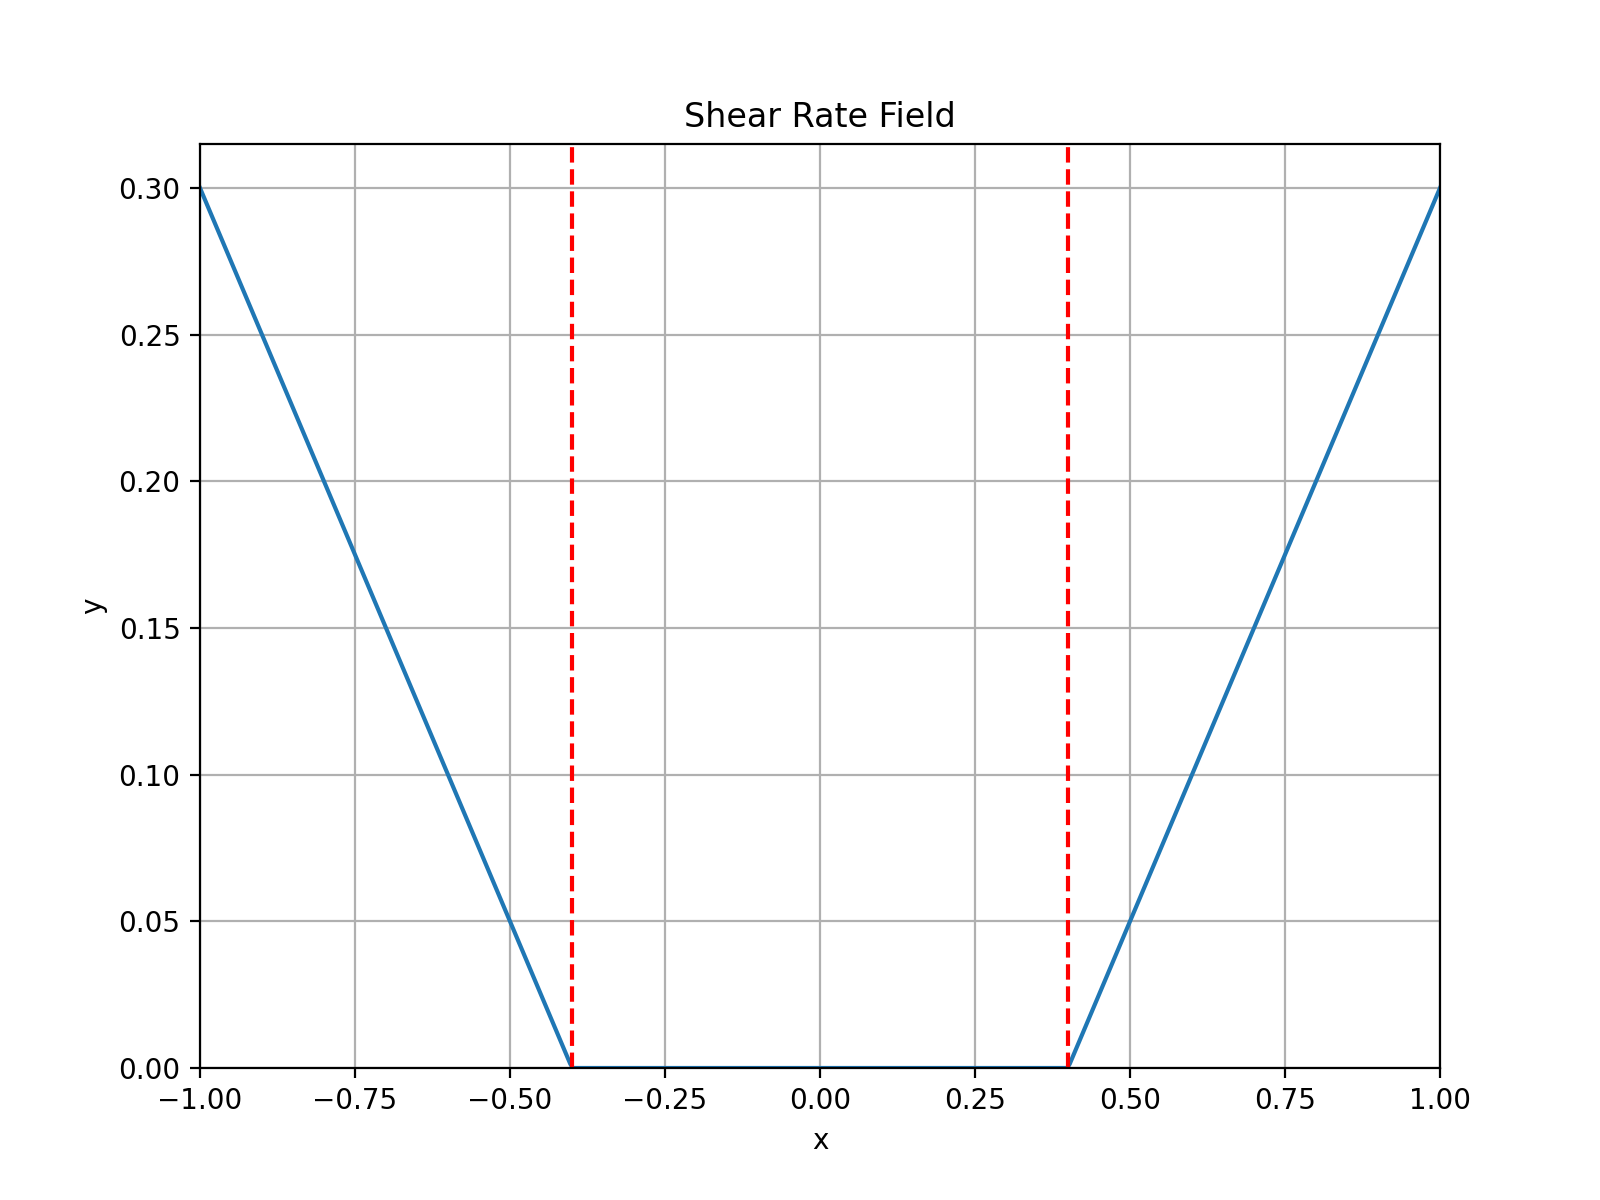
\includegraphics[width=0.8\textwidth]{figures/shear_rate_field.png}
%	\caption{Shear rate field for a Bingham fluid flowing through a tube.}
%\end{figure}
%\begin{figure}[ht]
%	\centering
%	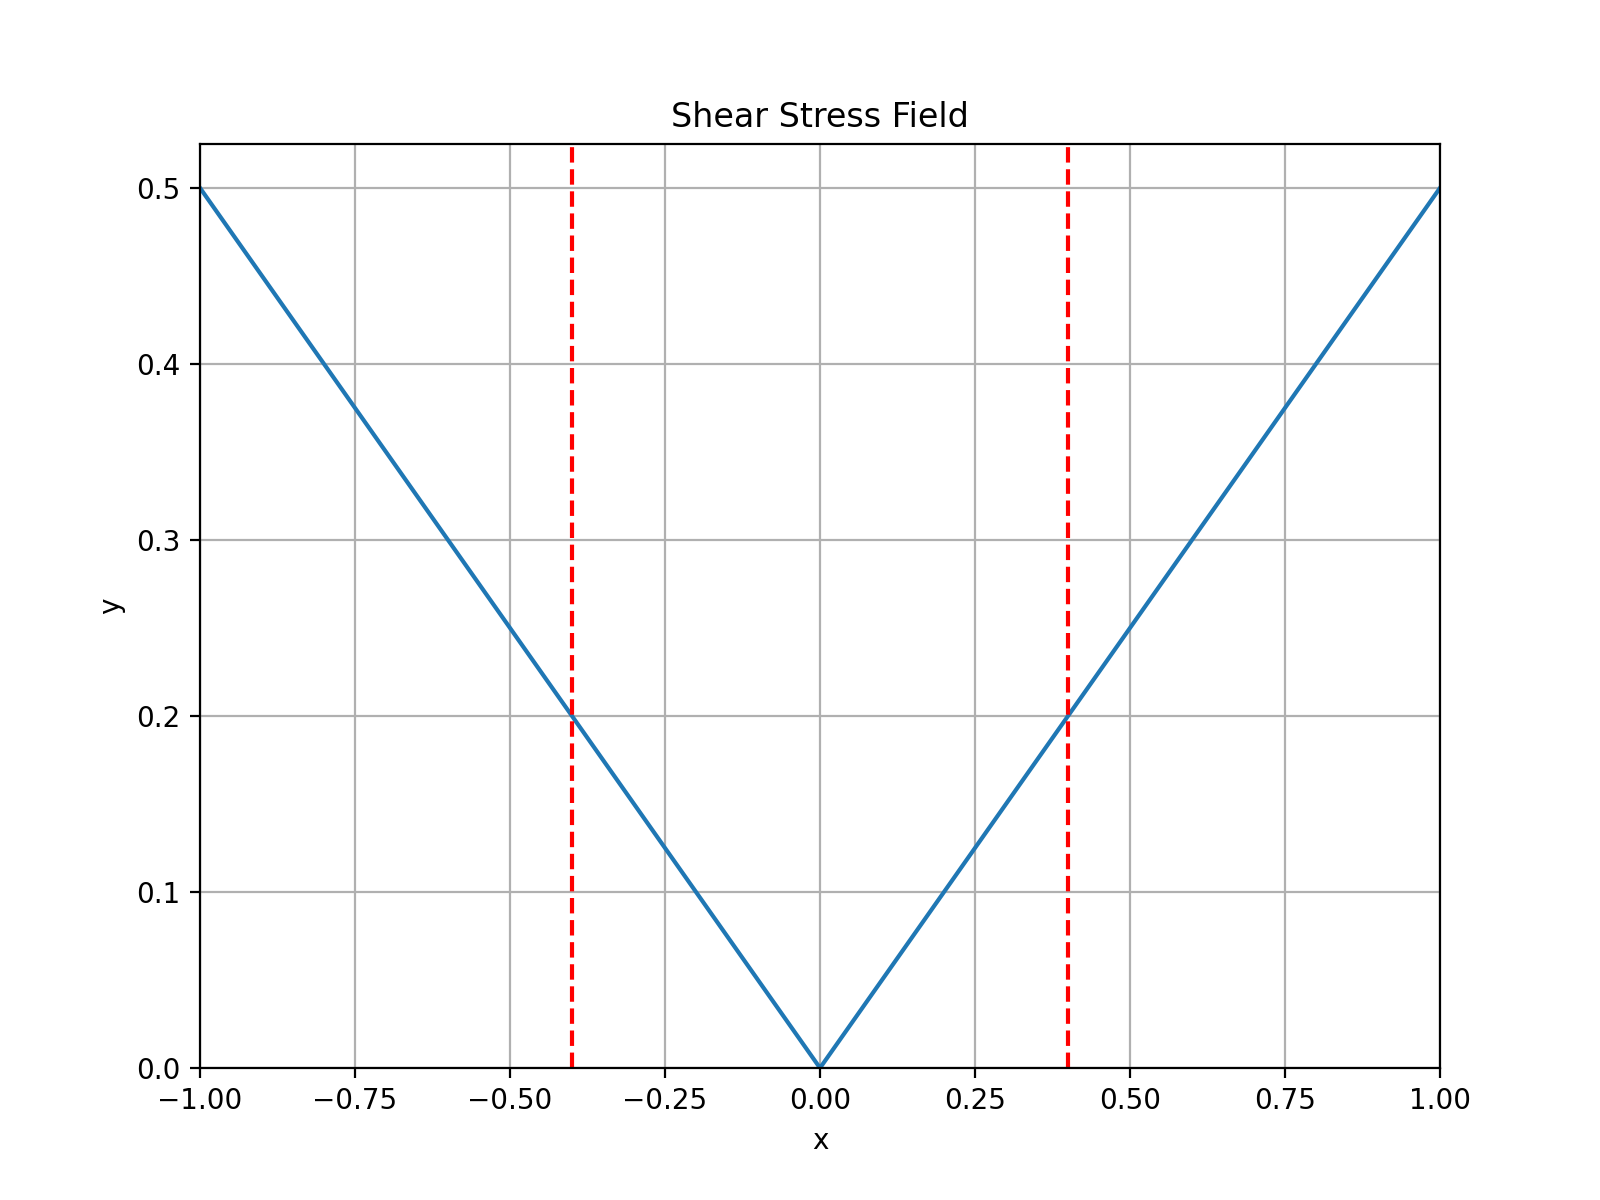
\includegraphics[width=0.8\textwidth]{figures/shear_stress_field.png}
%	\caption{Shear stress field for a Bingham fluid flowing through a tube.}
%\end{figure}
\begin{figure}[H]
	\centering
	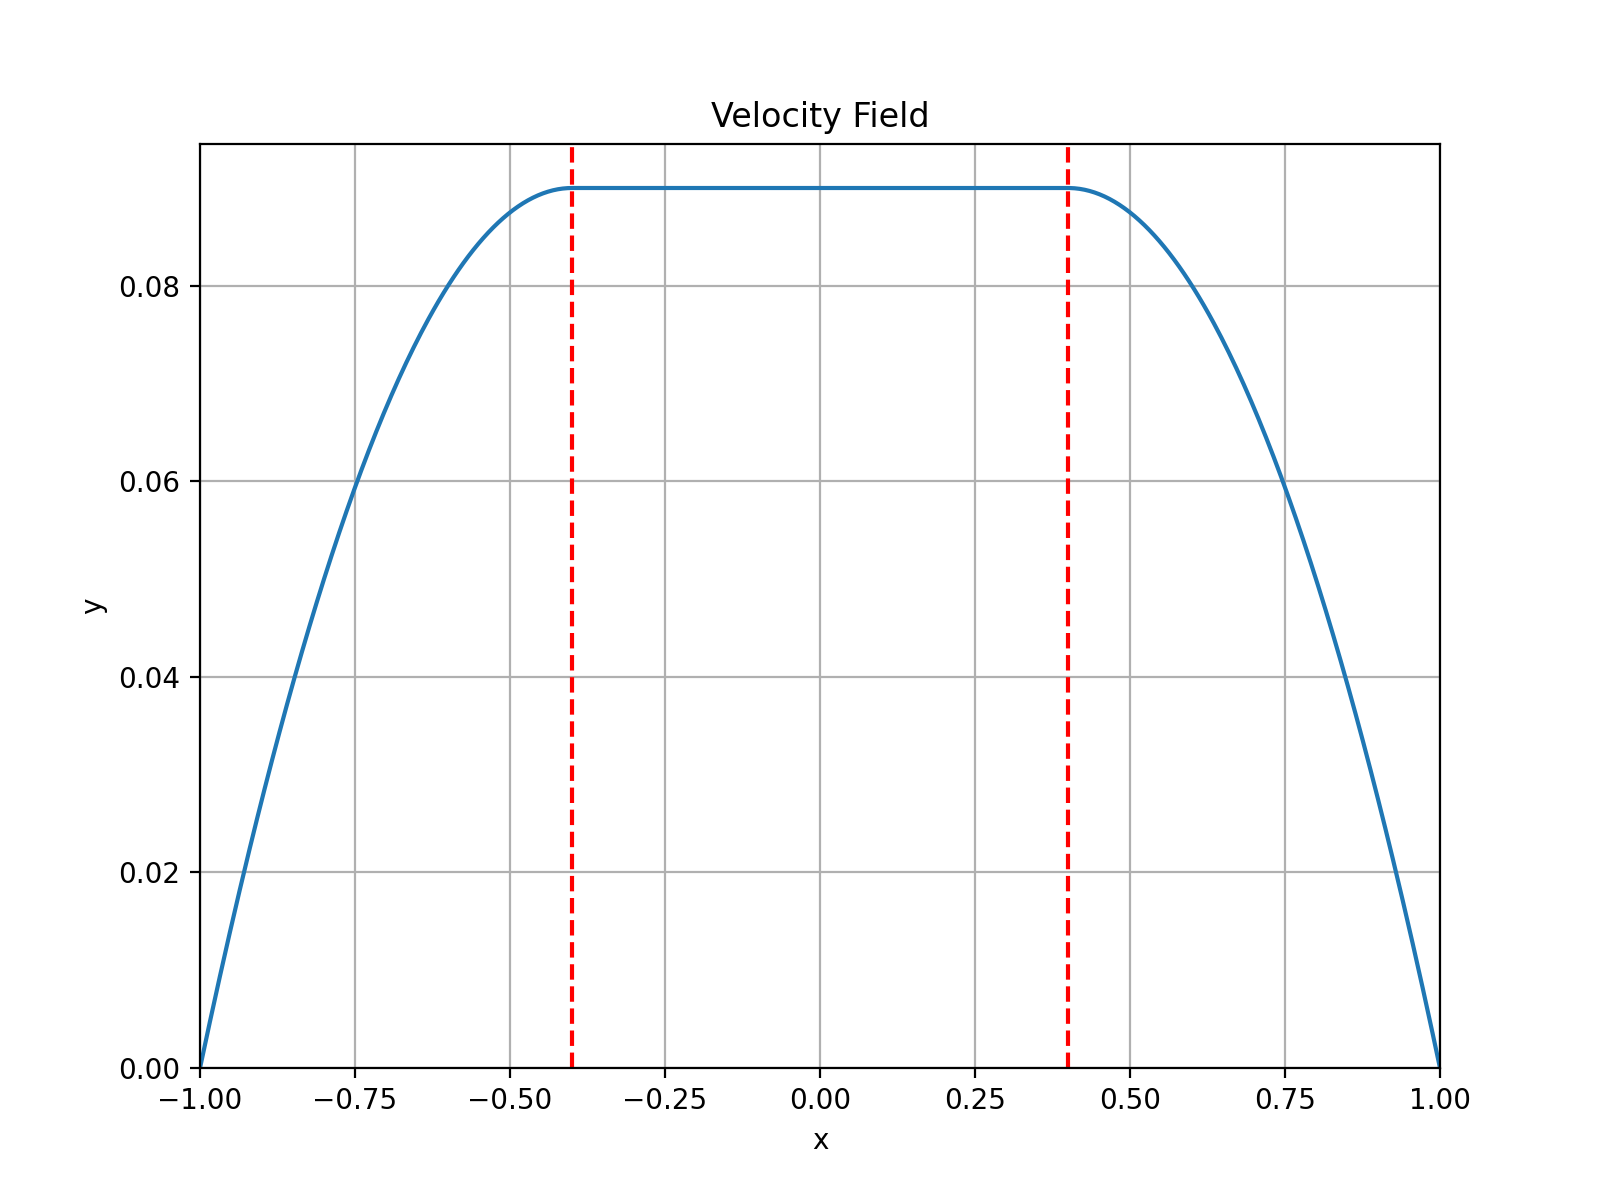
\includegraphics[width=0.8\textwidth]{figures/velocity_field.png}
	\caption{Velocity field for a Bingham fluid flowing through a tube.}
	\label{fig:malkin_3_9_velocity_field}
\end{figure}
\begin{figure}[H]
	\centering
	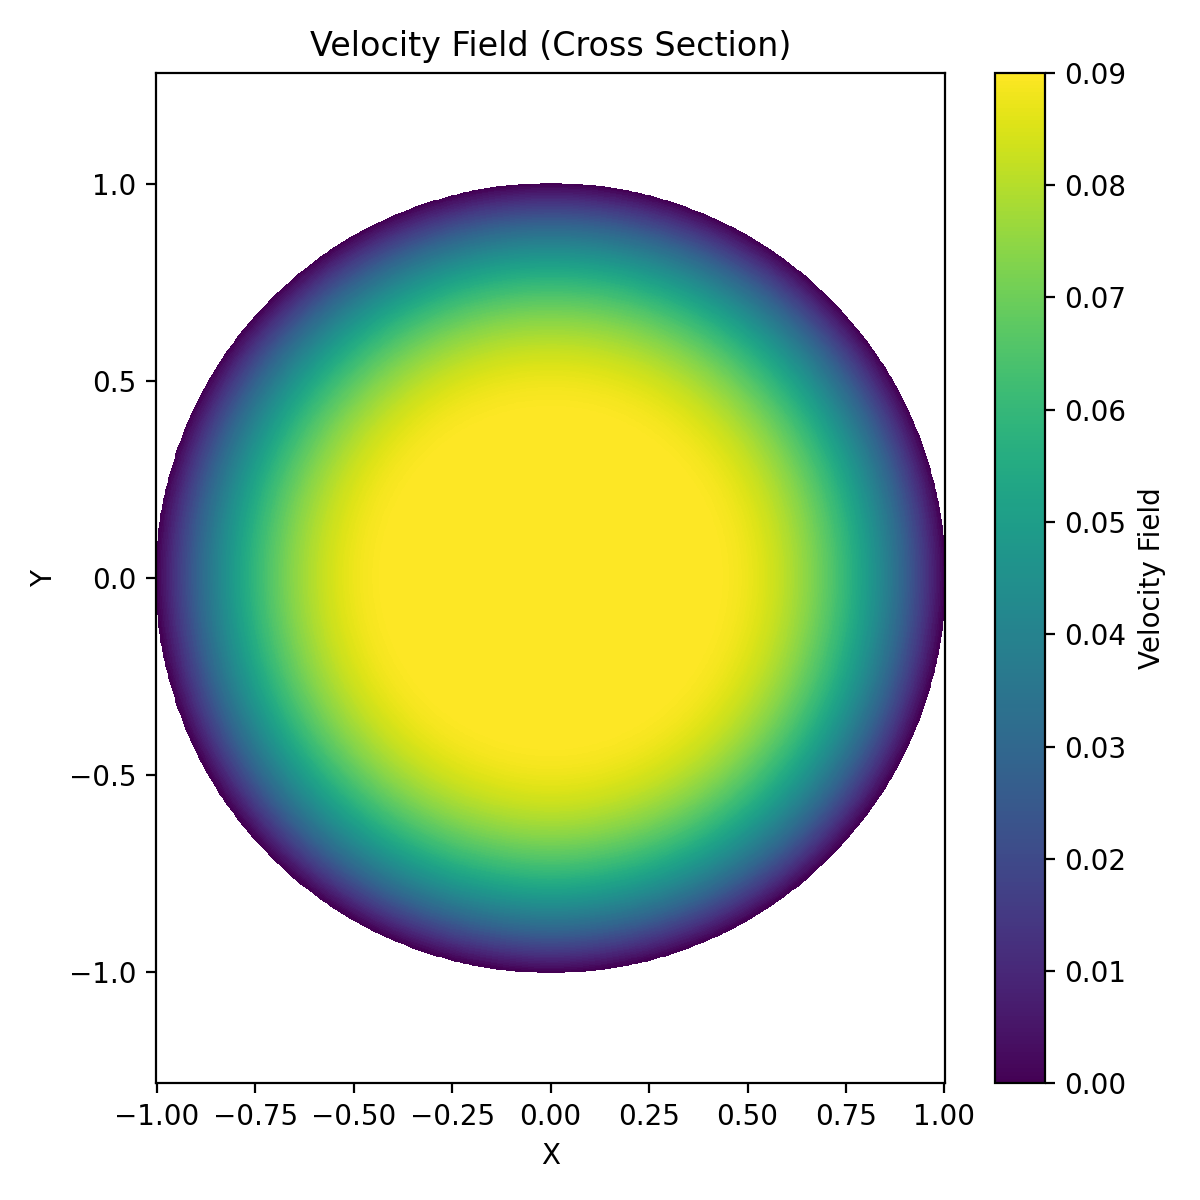
\includegraphics[width=0.32\textwidth]{figures/velocity_field_cross_section.png}
	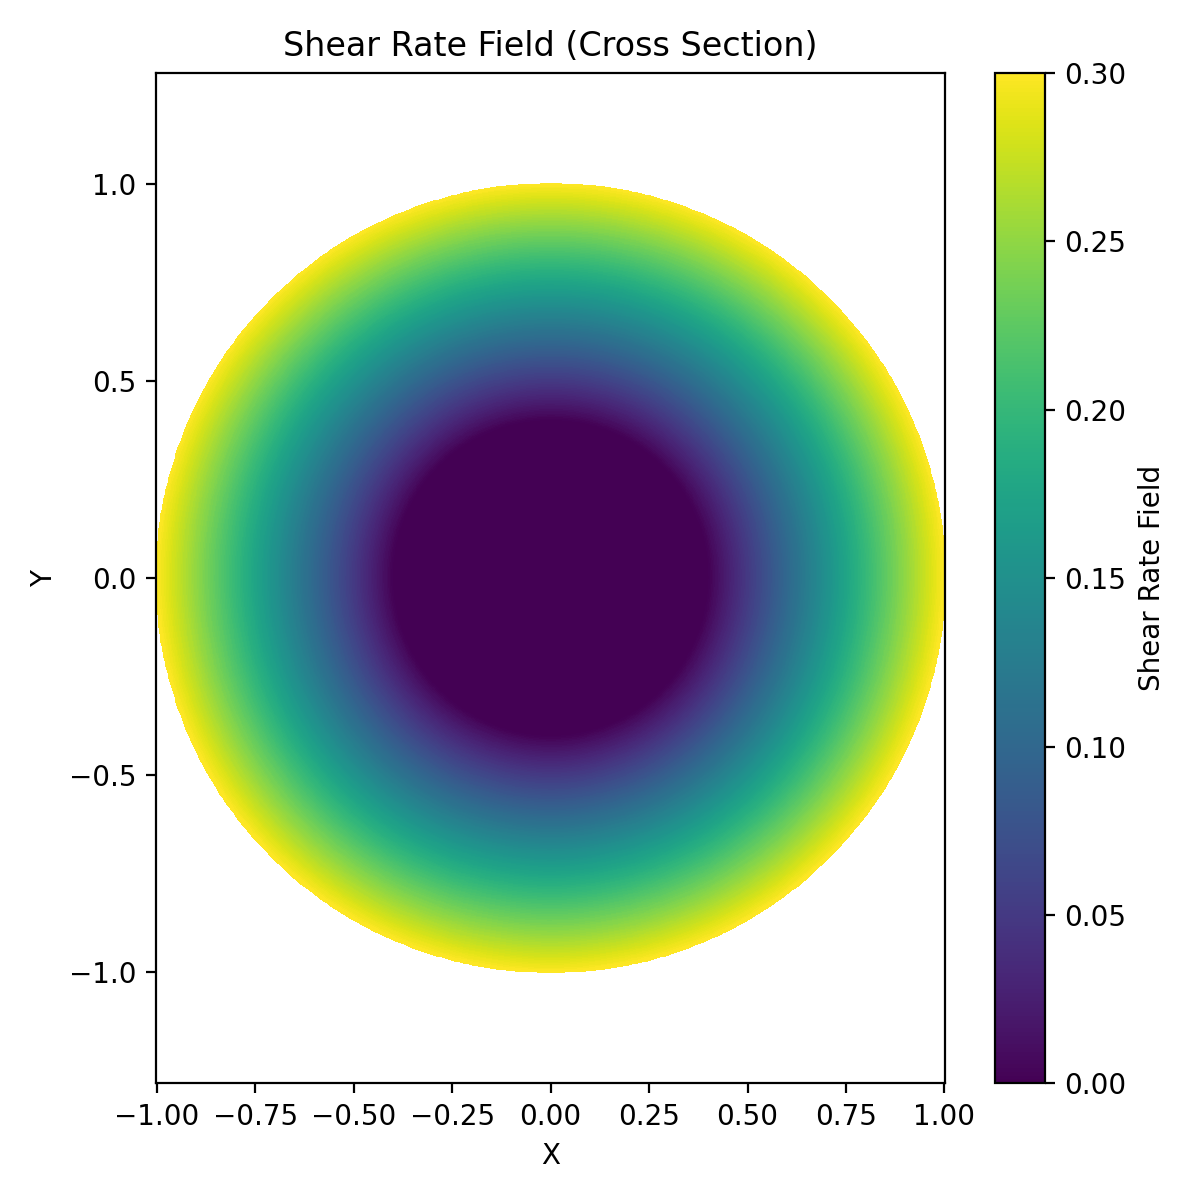
\includegraphics[width=0.32\textwidth]{figures/shear_rate_field_cross_section.png}
	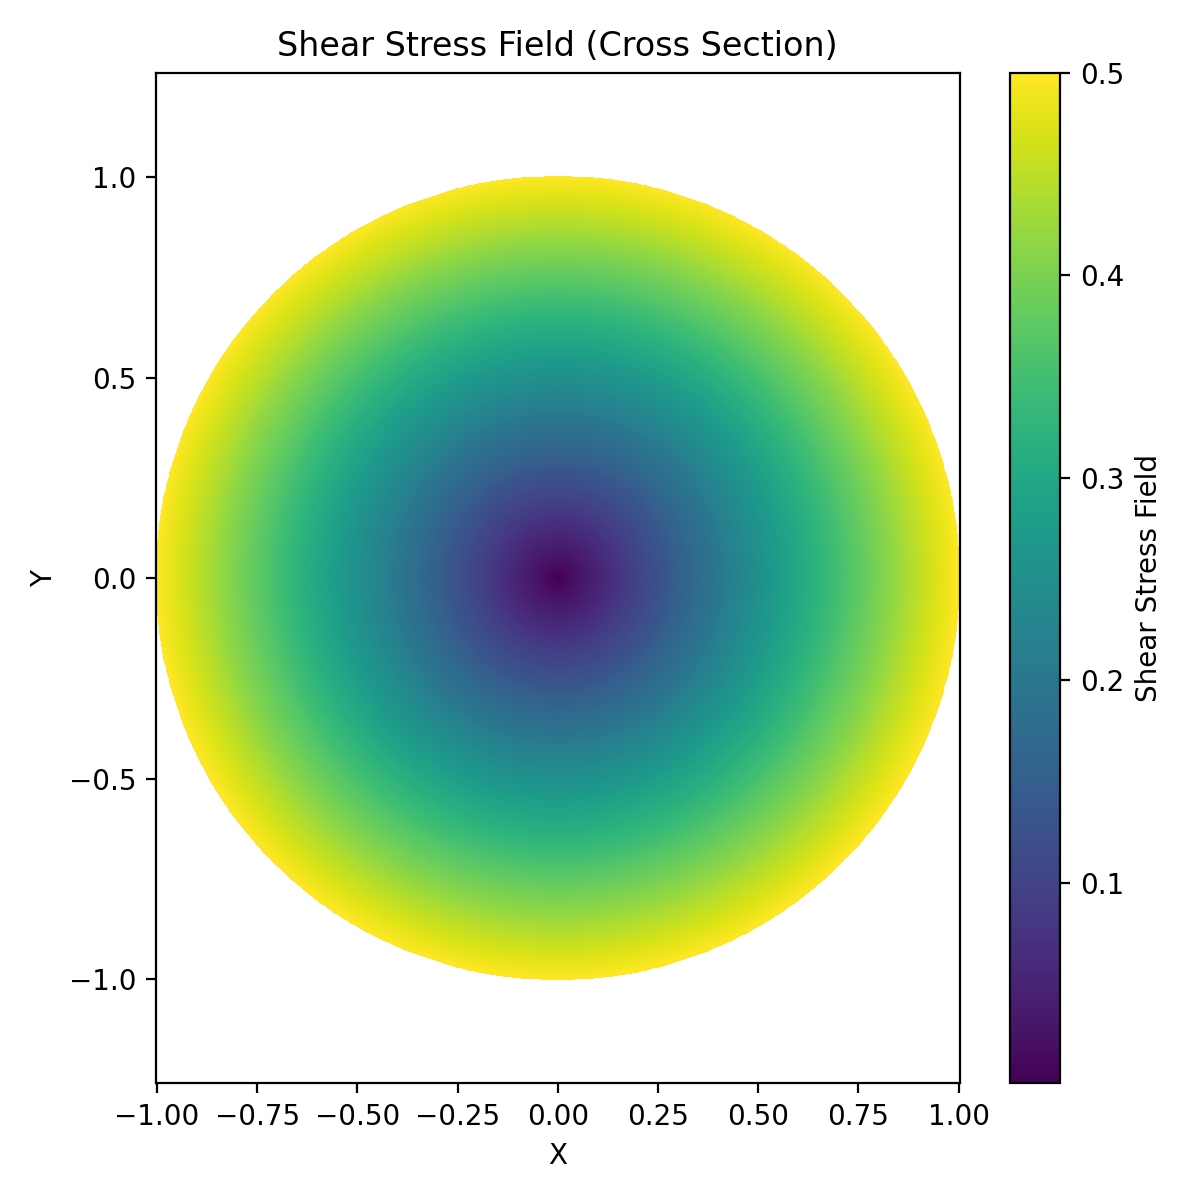
\includegraphics[width=0.32\textwidth]{figures/shear_stress_field_cross_section.png}
	\caption{Cross-sectional profiles of velocity, shear rate, and shear stress for a Bingham fluid flowing through a tube. The region near the center of the tube (where $r < r_0$) has zero shear rate. The velocity profile is flat in this region and then decreases towards the walls of the tube. The shear stress increases linearly with radius and exceeds the yield stress $\sigma_Y$ at $r = r_0$.}
	\label{fig:malkin_3_9_cross_section}
\end{figure} 



\subsection{3-10 Malkin}
A ball with a radius $R$ is falling in a Newtonian liquid having viscosity $\eta$. After some transient period, the velocity of ball movement becomes constant. Find the velocity of steady movement.

After talking to Dr. Kreplak, you do something like this:
\[
	\mathbf{F}_\text{net} = \mathbf{F}_\text{gravity} - \mathbf{F}_\text{drag} = 0.
\]
For a sphere, the drag force is given by Stokes' law:
\[
	mg = 6\pi \eta R v \implies v = \frac{mg}{6\pi \eta R}.
\]



\subsection{3-11 Malkin}
An experimenter measured the viscous properties of the material at different shear rates and obtained a flow curve. What can he say concerning viscous properties of this material in the uniaxial extension? Explain the answer.

\subsection{3-12 Malkin}
Prove the validity of Eq. 3.1.7 — the dependence between normal stress and deformation rate for Newtonian liquid in two-dimensional (biaxial) extension.

\subsection{3-13 Malkin}
Normal stresses in shear appear as a second-order effect. However, at high shear rates, they exceed shear stresses. Estimate the condition under which it becomes possible.

\subsection{3-14 Malkin}
Can normal stresses appear in the shear flow of suspension of solid particles? Explain the answer.

\textbf{Additional question.} Estimate the characteristic time (``relaxation time''), $\theta$, of this process.

\subsection{3-15 Malkin}
An experiment was carried out in shear at the constant shear rate, $\dot{\gamma}=\mathrm{const}$, and the curve similar to shown in Fig.~3.5.1 or Fig.~3.5.2 was obtained. Can the ratio $\sigma(t)/\dot{\gamma}$ be treated as the evolution of viscosity of liquid? Explain the answer.

\subsection{3-16 Malkin}
A liquid layer is intensively sheared at shear rate $\dot{\gamma}=1\times10^2\,\mathrm{s}^{-1}$. A liquid is Newtonian and its viscosity $\eta=500\,\mathrm{Pa\cdot s}$. Shearing continued for $10\,\mathrm{s}$. Temperature dependence of viscosity is neglected; density is assumed to be $1\,\mathrm{g/cm^3}$ and heat capacity is $0.5\,\mathrm{J/(g\cdot K)}$. What temperature rise is expected?

\textbf{Additional question.} If shearing proceeds for a longer time, what physical phenomena must be taken into consideration and what final thermal effect of shearing can be expected?

\subsection{3-17 Malkin}
Analyze the Mooney equation (3.3.27) for the concentration dependence of viscosity for the limiting case and, in particular, calculate the intrinsic viscosity of dilute suspensions.

\subsection{3-18 Malkin}
Newtonian viscosity of polymer with molecular mass $M_1=3\times10^5$ is $\eta_1=5\times10^5\,\mathrm{Pa\cdot s}$. There is also another polymer of the same chemical structure with molecular mass $M_2=4\times10^4$. How can one decrease the viscosity of the polymer by 10 times?

\subsection{3-19 Malkin}
Experiments show that an electrical charge appears on the surface of the polymer stream leaving a capillary in an unstable or spurt regime. Explain the origin of the charge.

